\chapter{Theoretical Introduction}


\section{Pain}

Pain is often defined as "an unpleasant experience which we primarily 
associate with tissue damage, or describe in terms
of such damage, or both" \cite{Fang2025}. Although pain affects the \ac{cns} directly, it also impacts the \ac{ans}, since it connects the \ac{cns} to the internal organs \cite{Moscato2022}.

According to its duration, pain can be classified as acute or chronic. Acute pain is induced by the activation of nociceptor sensory neurons, which occurs in the presence of actual or potential damaging stimuli, such as intense heat or cold and excessive mechanical force, or due to inflammation \cite{Jayakar2021}. On the other hand, chronic pain is defined as lasting more than three months \cite{Raman2022} and can be classified into nociceptive, neuropathic or nociplastic pain. Nociceptive pain results from continuous stimuli associated with tissue injury, while neuropathic pain results from damage to the peripheral or central nervous system. Lastly, nociplastic pain is a broader term, that is applied to chronic pain when it can't be described by the other two terms \cite{Fitzcharles2021}.

The Numerical Pain Scale is one of the most widely used traditional methods for assessing pain. It typically involves asking patients to rate their pain on a scale from 0 to 10, where 0 represents no pain and 10 signifies the worst pain imaginable \cite{Nugent2021}. While simple and easy to administer, this method relies entirely on the individual’s subjective interpretation of their pain, which can be influenced by factors such as mood, stress and gender, not allowing for viable continuous monitoring. Besides this, the difference between pain scores may not be comparable in scaling the intensity of pain \cite{Adeboye2021}. Finally, its verbal component is a limitation for non-verbal patients who may not be able to describe their pain using this method.

Another traditional method for assessing pain is the Visual Analogue Scale. This scale represents a continuous range of values, and it mainly uses a horizontal line measuring exactly 100 mm. The patient is asked to make a mark on the line according to their level of pain, then, the distance of the mark is measured and recorded in millimetres or centimetres \cite{Bielewicz2022}. However, even though it’s non-verbal, a minimum level of motor abilities is necessary to correctly use the VAS, which makes it inadequate for scaling pain in some patients with motor impairment, for example. This method, although it seems to be more detailed in values than the NPS, is still very subjective, not allowing for an accurate pain description and comparison. This method can also be used for assessing other symptoms, however. For example, in the dataset used in this project, it was used to assess the level of anxiety, happiness, fear and stress that the participants felt, on a scale of 0-100\%, and the arousal and valence states in a -5 to 5 scale \cite{Alves2024}.

Other similar scales, that also depend on a patient's perception of their own pain, end up also being subjective \cite{Adeboye2021}\cite{Robinson2024}. Due to this, researchers have attempted to find objective ways to describe pain using physiological signals.


\section{Pain Description}

The premise that pain induces changes in the \ac{ans} has led to the idea that physiological measures can be used to describe it \cite{Rojas2023}. For this reason, multiple physiological signals have been analysed in an attempt to select features that distinguish pain from the lack of it, or even classify it as more or less severe. 






\subsection{Electrocardiogram}

In this project, the chosen physiological signal was the \ac{ecg}.

The heart functions as a pump, its activity determined by the sinus node, that transmits excitation to the atrium and ventricule successively. An \ac{ecg} provides a recording of this electrical activity. Alterations in the typical conduction of electrical impulses through the heart can be detected on an \ac{ecg} and may reflect underlying physiological changes in the individual \cite{Liu2022}.

The \ac{ecg} signal can be segmented into successive waveforms that exhibit a consistent pattern and, therefore, it's possible to split those into specific components. The P wave surges as a result from the depolarization of the atrium. This electrical impulse spreads to the ventricule during the P-R segment and, as the ventricular muscle contracts, the QRS complex appears. Lastly, after the S-T segment, the T wave matches the repolarization of the ventricule \cite{hampton2024ecg}. These waves are shown in Figure \ref{fig:esquemaecg}, as well as other divisions, such as the P-R and S-T intervals. The onset of the P and T waves match the beginning of the P-R interval and the end of the S-T segment, while their offset corresponds to the start of the P-R segment and the end of the S-T interval, respectively. Similarly, the onset and offset of the R wave coincide with the start and end of the QRS complex \cite{Zhang2024}.

\begin{figure}[h!]
    \centering
    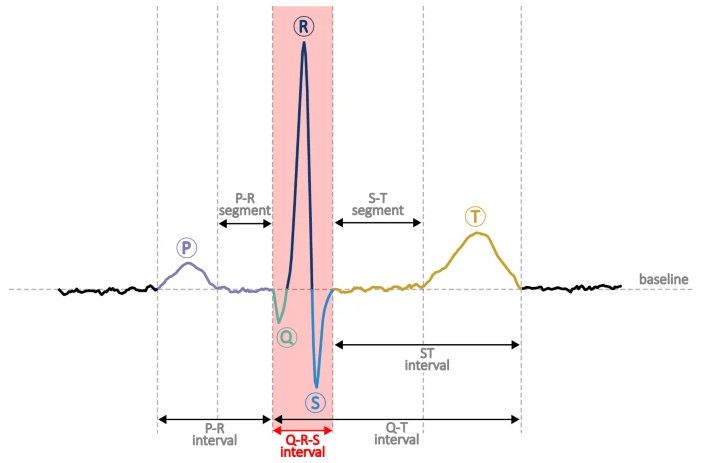
\includegraphics[width=0.7\textwidth]{esquema ECG.png}
    \caption{\ac{ecg} Schematic (Adapted from \cite{Dogan2023})}
    \label{fig:esquemaecg}
\end{figure}


\subsection{Related Works}

%The most popular signal that is used to describe pain is \ac{eda}, which measures skin conductivity, reflecting sweat gland activity, since it is related to the Sympathetic Nervous System \cite{Rojas2023}. - falar de SCL e GSR

In literature, the most common feature extracted from the \ac{ecg} is \ac{hrv}, which is related to time variations in R-R intervals. Nevertheless, other \ac{ecg} features have been analysed and selected as successful pain descriptors, along with features extracted from different physiological signals, like the \ac{emg} and \ac{eda}. For this signals' analysis, various machine learning models have been used, having achieved successful results throughout the years \cite{Moscato2022}\cite{Pais2025}.

For example, Pavlidou and Tsiknakis \cite{Pavlidou2025} used the BioVid Heat Pain dataset, in which heat pain was induced through a thermode, with the intent of obtaining significant features for pain classification. On that account, they extracted features from the \ac{ecg}, \ac{emg} and \ac{gsr} from 87 participants, where the first are HRV related. To detect pain, \acp{svm} and \ac{lstm} models were created while a \ac{loso} cross validation method was used to evaluate its intensity, distinguishing between a \ac{bl} and four levels of pain intensity (PA1, PA2, PA3 and PA4). The highest accuracy was obtained for multimodal approaches, with a maximum accuracy of 76.69\% for \ac{svm} and 77.21\% for \ac{lstm}. However, in unimodal approaches, \ac{gsr} features led to the best results, when compared with the other signals. Finally, the \ac{loso} method achieved a maximum accuracy of 82.83\% in \ac{bl} versus PA4, in accordance with the remaining results, where the best classification matched the models that compared the highest and lowest level of pain or the \ac{bl}.

Silva and Sebastião \cite{Silva2023} used a \ac{cpt} to induce pain in 36 participants, while eliciting distinct emotions through fear-inducing and neutral videos across two different sessions. This was done with the aim of measuring the effect of emotional contexts on physiological responses to pain. During the study, \ac{emg}, \ac{ecg}, \ac{eda}, and \ac{bp} data was collected. However, only the \ac{ecg} signals were analysed, using sliding windows for feature extraction. Subsequently, a variety of machine learning algorithms, including AdaBoost, Decision Trees, \ac{knn}, Linear Discriminant Analysis, Logistic Regression, \ac{rf}, and \acp{svm}, were employed across three classification strategies: dependent, session-independent, and participant-independent approaches. In the first, a maximum balanced accuracy of 97.4\% was obtained, while the second reached 97.7\% of balanced accuracy, which supports the hypothesis that the physiological response to pain remained consistent despite differing emotional contexts. Across the three approaches, the \ac{rf} and Adaboost models attained the best results. Meanwhile, the most relevant features were the amplitude of the S peaks, the amplitude of the T peaks, the amplitude of the T offset, and the amplitude of the R peaks. Although emotion elicitation was intended, self-reported pain levels did not reveal statistically significant differences between the fear and neutral sessions. This result was attributed to patients being too focused on the pain to pay attention to the video.

Choosing an alternative approach, Balasubramani et al \cite{Balasubramani2025} analysed \ac{ecg} signals from 142 patients who underwent surgical procedures. Their methodology involved using two dimensional Continuous Wavelet Transform on the signals, and processing the results through a framework that combines a quantum neural network architecture and classical deep learning models. This new model achieved an accuracy of 94.8\% in pain assessment, implying that quantum transfer learning might acquire a fundamental role in future medical diagnostic systems. 






